
\begin{teaserfigure}
	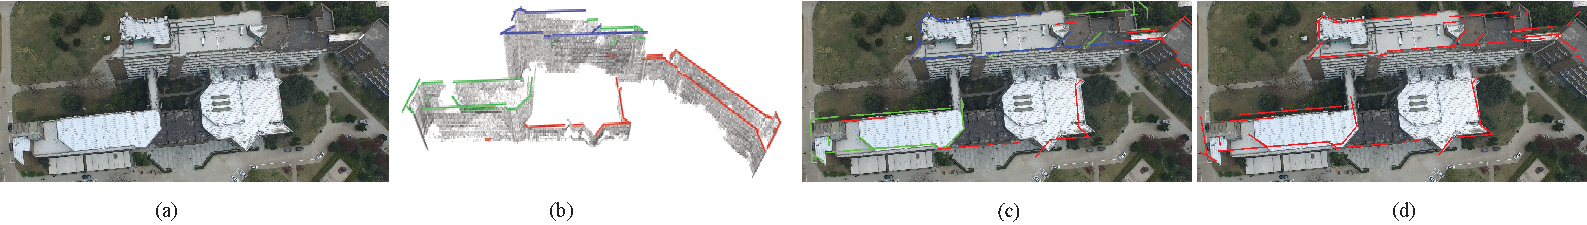
\includegraphics[width=\textwidth]{figures/new_teaser_pdf}
	\caption{(a) The overhead image is captured by an aerial device in a low altitude. (b) The point cloud is scanned by a laser device on the ground. We extract the roof contours (in different colors) according to the altitude histogram of points (c) The contours are matched with the overhead image respectively to achieve an initialization for optimizing the global matrix. (d) The camera pose is estimated after the iterative global matrix optimization. We project the contours on the overhead image to show the results.}
	\label{fig:teaser}
\end{teaserfigure}


\maketitle



\section{Introduction}
%
As a key technique to image-based navigation, augmented reality, 3D city modeling and so on, geo-localization has drawn massive attentions in the literature. 
%
The geo-localization problem is defined as aligning an image with a 3D model to estimate the camera pose \md{ with respect to the global coordinate of the 3D model.} \cxj{of what? Whose global coordinate?}.
%
The sensor prior\md{, including the compass and GPS, }\cxj{including what? be specific} is optionally employed. 

\cxj{Then talking about previous methods.}
\md{There are two typical types of images are used in geo-localization systems. 
%
One is the facade-view image captured on the ground~\cite{Arth}. 
%
The other one is remote sensing image captured in significantly high altitude~\cite{Liu, Zhang}.} \cxj{Do we need more references?}
%
\cxj{Discuss more about their methods.}
%


\cxj{Our method}
%
\cxj{What is the motivation of using overhead-image?}
With the populization of consumer-level drones, low-altitude overhead images can be easily obtained for buildings.
%
In this work, we estimate the camera pose using an overhead image captured by a low-altitude aerial device as query and a corresponding building point cloud as 3D model. 
%
The building point clouds we deal with are scanned by a laser device, and only facades of buildings are able to be scanned. 
%
Comparing to existing methods using images captured on the ground~\cite{Arth} or in high altitude~\cite{Karl, Zhang}, we face challenges that we are not able to take advantages of vanishing points in overhead image and suffer from more critical perspective effect in low-altitude image. 

\md{To build the correspondence between the overhead image and the point cloud scanned on the ground, we observe that: 1) vertical facades of a point cloud correspond to edges of building roofs in the overhead image; 2) roofs of different altitudes are in different scales in the overhead image due to perspective projection. Based on these two observations, we solve this geo-localization problem with a combination of a multi-layer shape matching problem and a global optimization of camera pose estimation.}

\cxj{Our method is able to handle various types of scenes, including .. overhead images containing partial buildings. }
%利用这个方法,我们可以。。。。。
%
\begin{figure}[t]
	\centering
	%\vspace{2.0cm}
	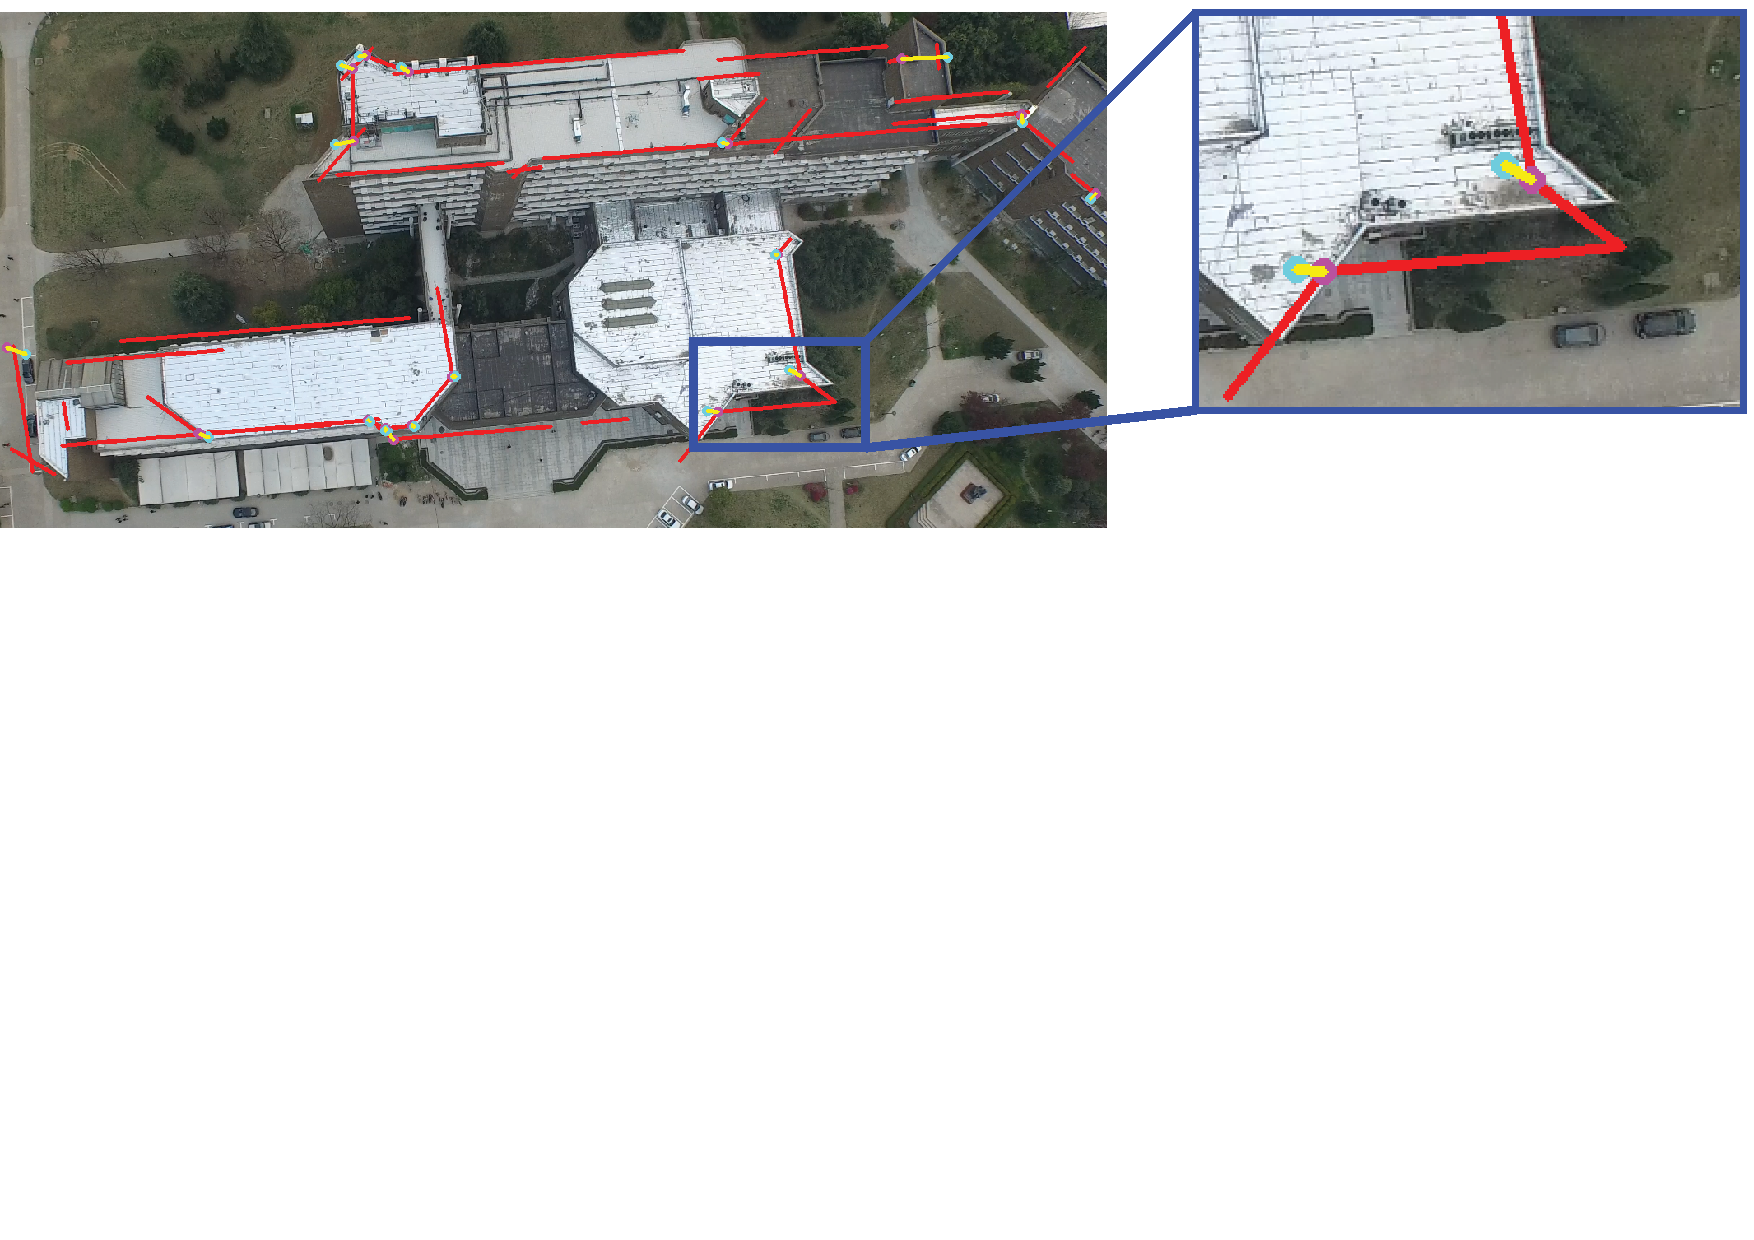
\includegraphics[width=0.5\textwidth]{figures/details_pdf}
	\caption{Finding paired 3D and 2D feature points: for a 3D feature point, we project it on the overhead image (magenta points) using current project matrix and search in its $k\times k$ neighborhood for a corner (cyan points). These 3D feature points and corresponding corners form pairs of feature points for next iteration of calculating project matrix.}
	\label{fig:overview}
\end{figure}




\section{Our Approach}
\md{
Given an overhead image and the point cloud of a building, our method consists of two parts. 
%
The first part is a shape matching between the 3D contours of the point cloud at multiple sampled altitudes and the edges in the overhead image, as Figure~\ref{fig:teaser}(b)(c) show. 
%
The second part is a global optimization of the camera pose by refining point correspondences based on the shape matching results, as Figure~\ref{fig:teaser}(d) shows. 
}

\paragraph{Shape Matching.}
%
\md{The vertical directions of point clouds we use are aligned to the gravity direction in the reality. If this is not satisfied, a technique of finding the up-vector based on principle component analysis (PCA)~\cite{Karl} can be used to rotate the point cloud to meet the alignment.}
We divide the point cloud into several part vertically \md{by sampled altitudes determined by sharp changes in the altitude histogram of points}. \cxj{The sampling interval is determined ... as what?}
\md{In each interval, points are vertically projected to the upper cross section and fitted into 2D line segments on the cross section using a RANSAC line fitting algorithm.} \cxj{using the ... algorithm}.
%
Taking line segments at each altitude as a contour of a building roof, we match contours with the edge map of the overhead image respectively using a shape matching technique~\cite{Zhang}. 
\cxj{Directly use the shape method without any modification? The same matching objective function with the reference? }
%
A local project matrix is achieved for each contour after shape matching. The project matrix is defined as $\mathbf{M_0}=\mathbf{K_0[R_0|T_0]}$, where $\mathbf{K_0}$ is the pre-calibrated intrinsic camera matrix, $\mathbf{R_0}$ is a $3\times3$ rotation matrix, and $\mathbf{T}$ is a 3-D translation vector. Here $\mathbf{R_0}$ is a 1 degree-of-freedom (dof) matrix since we assume that the optical axis of the camera is aligned to the vertical direction of the point cloud and only the rotation of the vertical direction is needed to be estimated. The assumption will be discarded in global optimization part.

\md{From Figure~\ref{fig:teaser}(c), we can see that the 2D shape matching generates a rough alignment between the contours and the overhead image. However, there are obvious deviation at corners due to the non-ideal perpendicular projection of the low-altitude camera.}
%
Therefore, we need a global project matrix instead of local ones to estimate the camera pose. 
So we treat the results of shape matching as the initialization of following global optimizing procedure. 


\paragraph{Global Optimization.}
%
\md{
We define the global project matrix from the 3D point cloud to the image as $\mathbf{M}=\mathbf{K[R|T]}$, where $\mathbf{K}$ is the intrinsic camera matrix, $\mathbf{R}$ is a 3 dof rotation matrix, and $\mathbf{T}$ is a 3-D translation vector. }
%
To calculate the global project matrix, we first find a set of paired 3D feature points and corresponding 2D feature points. 
%
For 3D feature points, we take the intersections of adjacent line segments of the contours. 
%
And then we employ an iterative algorithm to optimize the global project matrix by alternatively finding corresponding 2D feature points and calculating the project matrix, where we utilize the results of shape matching as initial project matrix.
 

To be more specific, we apply two steps in every iteration alternatively until the convergence. 1)~As shown in Figure~\ref{fig:overview}, for a 3D feature point $\mathbf{x}$ we project it on the overhead image using current project matrix to get a 2D point $\mathbf{q}$ (Cyan points). We then search its $k\times k$ neighborhood for a 2D corner $\mathbf{p}$ with the maximum Harris corner response (yellow points). 
\md{We set $k=31$ in all our experiments.}
%
%
%These 3D feature points and corresponding corners form paired feature points for the next step of calculating project matrix.
%Once a set of paired 3D and 2D feature points is achieved, we randomly select a subset of these feature point pairs to calculate a global matrix. 
2) With a set of paired 3D and 2D feature points, we can optimize the global project matrix $\mathbf{M}$ by minimizing the average of distances of pixels between projected contours and the edges of the overhead image, which can be accelerated by distance transformation. 
%
And the newly calculated project matrix is used for the next iteration of finding paired feature points.
%

With the optimized global project matrix and focal length of the camera, we can finally estimate the 6 dof camera pose of the overhead image in point cloud coordinate system.
\cxj{So you do not refine the camera intrinsic parameters?} \lyh{We need focal length to determine the translation of z.}

% Be more specific?
\section{Experiments and Future Work}
%We tested the proposed approach on a newly collected dataset, which contains several low-altitude overhead images and corresponding building point clouds. Figure 3 shows one of the results and a comparison of some details of the result, where we project roof contours on the overhead image. As we can see, the result after the global optimization is not much more accuracy than that before the global optimization.
We tested the proposed approach on \md{wide range of buildings}. 
\md{We scanned 10 buildings in our campus using a laser 3D scanner}. 
A group of overhead images are captured by a drone.\cxj{proide the specific model.}
%
Figure~\ref{fig:comparison} shows the results of our experiments, where we project roof contours on the overhead image based on the estimated camera poses. 
%
\md{We can see that our method is able to accurately align the over-head images captured at different positions with various buildings. The buildings are irregular, consisting parts of various heights.  }

%The proposed method uses the results of shape matching stage as the initialization of the global optimization stage. We find that the global optimization can correct some small mistakes taken in shape matching stage. 

\md{The average time of register an $1300\times 600$ overhead image to a 3D point cloud containing about $300K$ 3D points is about $8$ minutes.  }
\cxj{Check the numbers.}
%
In the future, we intend to implement a faster version of the algorithm using parallel computing.
%
Another future direction is camera tracking of a video sequence taking from overhead. This is useful for many drone-based applications.

\begin{figure}[b]
	\centering
	%\vspace{2.0cm}
	\includegraphics[width=0.5\textwidth]{figures/results_pdf}
	\caption{(a) The low-altitude overhead images. (b) Building point cloud with contours we extract. (c) Results of our experiments. We project the contours on the overhead image to show the results. \cxj{Why not use different colors for contours like in (b)?}}
	\label{fig:comparison}
\end{figure}
